\documentclass[11pt,a4paper]{article}

\usepackage[utf8]{inputenc}
%\usepackage[english]{babel}
\usepackage{amsmath}
\usepackage{amsthm}
\usepackage{amssymb}
\usepackage{hyperref}
\usepackage{url}
\usepackage{mathtools}
\usepackage{tikz}
\usepackage{array}
\usepackage{pifont}
\usepackage{makecell}
\usepackage{csquotes}
\usepackage{pdflscape}
\usepackage{tabularx}
\usepackage{geometry}
\usepackage[graphicx]{realboxes}
\usepackage[ngerman]{babel}



\newcommand{\cmark}{\ding{51}}
\newcommand{\xmark}{\ding{55}}

\usetikzlibrary{arrows}
\hypersetup{
    colorlinks=true,
    linkcolor=blue,
    filecolor=magenta,      
    urlcolor=blue,
    citecolor=blue,
    pdftitle={Overleaf Example},
    }
\usepackage{listings}
\usepackage{xcolor}
\definecolor{delim}{RGB}{20,105,176}
\definecolor{numb}{RGB}{106, 109, 32}
\definecolor{string}{rgb}{0.64,0.08,0.08}
\definecolor{comment}{RGB}{123,188,123}
\definecolor{greencomment}{RGB}{0,128,0} % Define the green color for comments

\lstdefinelanguage{json}{
    numbers=left,
    numberstyle=\small,
    frame=single,
    rulecolor=\color{black},
    showspaces=false,
    showtabs=false,
    breaklines=true,
    postbreak=\raisebox{0ex}[0ex][0ex]{\ensuremath{\color{gray}\hookrightarrow\space}},
    breakatwhitespace=true,
    basicstyle=\small,
    upquote=true,
    morestring=[b]",
    stringstyle=\color{string},
    literate=
     *{0}{{{\color{numb}0}}}{1}
      {1}{{{\color{numb}1}}}{1}
      {2}{{{\color{numb}2}}}{1}
      {3}{{{\color{numb}3}}}{1}
      {4}{{{\color{numb}4}}}{1}
      {5}{{{\color{numb}5}}}{1}
      {6}{{{\color{numb}6}}}{1}
      {7}{{{\color{numb}7}}}{1}
      {8}{{{\color{numb}8}}}{1}
      {9}{{{\color{numb}9}}}{1}
      {\{}{{{\color{delim}{\{}}}}{1}
      {\}}{{{\color{delim}{\}}}}}{1}
      {[}{{{\color{delim}{[}}}}{1}
      {]}{{{\color{delim}{]}}}}{1},
      morecomment=[l]{\#}, % Define the '#' character as the start of a comment
      morecomment=[s]{\#}{\ }, % Define the end of the comment
      commentstyle=\color{greencomment}, % Set the color for the '#' and the following word
}

\usepackage{graphicx}
\graphicspath{{./images/}}


\newcounter{Figcount}
\newcounter{tempFigure}

\newenvironment{TableCaption}{%
    \renewcommand{\figurename}{Table}
    \setcounter{tempFigure}{\thefigure}
    \setcounter{figure}{\theFigcount}
    }{%
    \setcounter{figure}{\thetempFigure}
    \stepcounter{Figcount}
    }


\numberwithin{equation}{section}
\newtheorem{definition}{Definition}[section]
\newtheorem{example}{Example}[section]
\newtheorem{satz}[definition]{Satz}
\newtheorem{lemma}[definition]{Lemma}
\newtheorem{fact}[definition]{Fact}

\title{Philipps-Universität Marburg\\[0.0em] Fachbereich Mathematik und Informatik\\[0.0em] AG Softwaretechnik \\[0.0em] \textbf{Analysis of Conflicts and Dependencies between User Stories}\\[0.0em]}
%\title{Philipps-Universität Marburg\\  }
%\large{Masterarbeit} \\ zur Erlangung des akademischen Grades\\ Master of Science \\ \\ \\ vorgelegt von \\ \textbf{Amir Rabieyan Nejad} Matrikel-Nr: 3350269 \\}

\author{Amir Rabieyan Nejad}

\date{\today}
\thispagestyle{empty}

\begin{document}

\maketitle
\thispagestyle{empty}
\newpage\phantom{blabla}
\thispagestyle{empty}
%\begin{abstract}
%%benefit of graph transformation
\newpage
\section*{ Abstract}
\emph{User stories} (USs), the basic building blocks of software development, serve as precise and testable descriptions of a software's functionality. Within the dynamic framework of \emph{agile development}, these USs become a frequently used requirements notation in agile projects\cite{wang2014role}, which is usually written informally in plain text and managed in the \textit{product backlog}, which serves as a repository for prioritising and tracking development tasks.

As the amount of USs increases, conflicts or redundancies between them are inevitable. If a user story (US) requires the deletion of a component that is essential for the successful execution of another US, we are dealing with a conflict, or if a US (or some elements or parts of it) is a syntactic duplication of another US, we are dealing with redundancy.

In addition, changing an existing requirement or adding a new requirement to the existing product backlog in agile software development can also cause conflicts or redundancies due to changes in the needs and concerns of \emph{system stakeholders}. This can result in a wide range of inconsistencies, as requirements are raised by multiple stakeholders involved in product development to achieve different functions.

Effectively recognising these conflicts and redundancies is fundamental for development teams. By addressing these issues, teams can provide additional value to users, adapt to changing requirements and maintain consistency between USs. 

Normally, agile methods such as \emph{Scrum} encourage cross-functional collaboration and daily stand-up meetings as mechanisms to address and mitigate redundancies and conflicts in a timely manner. However, this approach can be time and resource consuming. In cases where the backlog is very extensive, recognising existing redundancies and conflicts between USs can become a complex undertaking.

Since there is no method for automatically identifying redundancies and conflicts between requirements written in natural language in agile software development, in this thesis, we want to present two approaches for analysing redundancies and conflicts between USs.

The first approach analyses redundancies by taking annotated USs as input (instead of US text) and using \textit{graph transformation} (GT), in particular \textit{Henshin} and its \textit{Conflict and Dependency Analysis} (CDA) tool, to detect potential redundancies in a syntactic way.

The second approach deals with analysing conflicts between USs, also using annotated USs as input. By utilizing \textit{Natural Language Processing} (NLP) technique, particularly VerbNet, and a specially implemented tool, we recognize potential conflicts in a semantic way.

We apply both approaches to 19 annotated backlog datasets and create comprehensive reports for each dataset. Upon evaluation, we find that the results of both approaches are satisfactory. However, we also notice that the quality of the USs and their annotations significantly influences the effectiveness of the results.

%\end{abstract}
%\section*{Selbstständigkeitserklärung}
Hiermit versichere ich, Amir Rabieyan Nejad, dass ich die vorliegende Arbeit mit dem Titel \emph{Analysis of Conflicts and Dependencies between User Stories using Graph Transformation} selbstständig verfasst und keine anderen als die angegebenen Quellen und Hilfsmittel benutzt habe. Die Masterarbeit wurde in der jetzigen oder ähnlichen Form noch bei keiner anderen Hochschule eingereicht und hat noch keinen anderen Prüfungszwecken gedient.

%\begin{figure}
\begin{flushleft}

\includegraphics[width=4.68cm, height=1.9cm]{1_signature}\\
\selectlanguage{ngerman}
Marburg, den \today
\selectlanguage{english}
\end{flushleft}
%\end{figure}







\newpage
%%benefit of graph transformation
\newpage
\section*{ Abstract}
\emph{User stories} (USs), the basic building blocks of software development, serve as precise and testable descriptions of a software's functionality. Within the dynamic framework of \emph{agile development}, these USs become a frequently used requirements notation in agile projects\cite{wang2014role}, which is usually written informally in plain text and managed in the \textit{product backlog}, which serves as a repository for prioritising and tracking development tasks.

As the amount of USs increases, conflicts or redundancies between them are inevitable. If a user story (US) requires the deletion of a component that is essential for the successful execution of another US, we are dealing with a conflict, or if a US (or some elements or parts of it) is a syntactic duplication of another US, we are dealing with redundancy.

In addition, changing an existing requirement or adding a new requirement to the existing product backlog in agile software development can also cause conflicts or redundancies due to changes in the needs and concerns of \emph{system stakeholders}. This can result in a wide range of inconsistencies, as requirements are raised by multiple stakeholders involved in product development to achieve different functions.

Effectively recognising these conflicts and redundancies is fundamental for development teams. By addressing these issues, teams can provide additional value to users, adapt to changing requirements and maintain consistency between USs. 

Normally, agile methods such as \emph{Scrum} encourage cross-functional collaboration and daily stand-up meetings as mechanisms to address and mitigate redundancies and conflicts in a timely manner. However, this approach can be time and resource consuming. In cases where the backlog is very extensive, recognising existing redundancies and conflicts between USs can become a complex undertaking.

Since there is no method for automatically identifying redundancies and conflicts between requirements written in natural language in agile software development, in this thesis, we want to present two approaches for analysing redundancies and conflicts between USs.

The first approach analyses redundancies by taking annotated USs as input (instead of US text) and using \textit{graph transformation} (GT), in particular \textit{Henshin} and its \textit{Conflict and Dependency Analysis} (CDA) tool, to detect potential redundancies in a syntactic way.

The second approach deals with analysing conflicts between USs, also using annotated USs as input. By utilizing \textit{Natural Language Processing} (NLP) technique, particularly VerbNet, and a specially implemented tool, we recognize potential conflicts in a semantic way.

We apply both approaches to 19 annotated backlog datasets and create comprehensive reports for each dataset. Upon evaluation, we find that the results of both approaches are satisfactory. However, we also notice that the quality of the USs and their annotations significantly influences the effectiveness of the results.

%%benefit of graph transformation
\section*{Zusammenfassung}
\emph{User Stories}, die Grundbausteine der Softwareentwicklung, dienen als präzise und testbare Beschreibungen der Funktionalität einer Software. Innerhalb des dynamischen Rahmens der \emph{agilen Entwicklung} werden diese User Stories in der Regel informell in einfachem Text verfasst und im \emph{Product Backlog} verwaltet, das als Repository für die Priorisierung und Verfolgung von Entwicklungsaufgaben dient.

\emph{Behaviour Driven Development} (BDD), ein spezieller Ansatz im Bereich der agilen Softwareentwicklung, legt einen starken Schwerpunkt auf die iterative Umsetzung von User Stories. Die Reihenfolge der User Stories im BDD ist ein zentraler Aspekt der Methodik. Die richtige Reihenfolge hat nicht nur Auswirkungen auf die Effizienz der Entwicklung, sondern auch auf den Gesamterfolg des Projekts. Durch eine effektive Priorisierung und Abfolge der User Stories können die Entwicklungsteams den Benutzern einen inkrementellen Mehrwert bieten, auf sich ändernde Anforderungen reagieren und sicherstellen, dass die kritischsten Funktionen zuerst behandelt werden.

User Stories sind oft voneinander abhängig, was zu potenziellen Konflikten führen könnte, wenn eine User Story die Löschung einer Komponente erfordert, die für die erfolgreiche Ausführung einer anderen User Story unerlässlich ist, oder wenn eine User Story ein Element einführt, das der Realisierung einer anderen User Story zuwiderläuft und diese somit verhindert. Darüber hinaus kann auch die Änderung einer bestehenden Anforderung oder das Hinzufügen einer neuen Anforderung zum bestehenden Product Backlog in der agilen Softwareentwicklung zu Konflikten führen, da sich die Bedürfnisse und Anliegen der Systemstakeholder ändern. Dies kann zu einer Vielzahl von Inkonsistenzen aufgrund widersprüchlicher Anforderungen führen, da Anforderungen von mehreren an der Produktentwicklung beteiligten Stakeholdern gestellt werden, um unterschiedliche Funktionen zu erreichen.

Um das Auftreten von Konflikten zu minimieren, sollten Teams in der Regel systematisch Abhängigkeiten zwischen User Stories innerhalb ihres Backlogs identifizieren und dokumentieren. Agile Methoden wie \emph{Scrum} fördern die funktionsübergreifende Zusammenarbeit und tägliche Stand-up-Meetings als Mechanismen, um Abhängigkeiten und Konflikte zeitnah anzugehen und zu entschärfen. Dieser Ansatz kann jedoch zeit- und ressourcenaufwendig sein. In Fällen, in denen das Backlog sehr umfangreich ist, kann das Erkennen bestehender Konflikte zwischen User Stories zu einem komplexen Unterfangen werden.

\emph{Modellbasiertes Software-Engineering} ist eine geeignete Methode, um die ständig steigende Komplexität von Softwareentwicklungsprozessen zu bewältigen. \emph{Graphen} und \emph{Graphtransformationen} haben sich als nützlich erwiesen, um solche Modelle und deren Änderungen zu visualisieren.

Da es in der agilen Softwareentwicklung keinen Prozess zur systematischen Identifizierung und Verwaltung von Konflikten zwischen in natürlicher Sprache erstellten Anforderungen gibt, soll in dieser Arbeit ein gut strukturierter Arbeitsablauf vorgestellt werden, der eine Sammlung von Techniken und Werkzeugen aus verschiedenen Bereichen verwendet, um die automatische Erkennung von Konflikten und Abhängigkeiten in natürlichsprachlichen User Stories zu beschleunigen.


\newpage
\tableofcontents
\newpage



\section{Introduction}\label{intro}
%We investigate methods for analysing quality of USs,  extracting domain models, applying graph transformation rules, and detecting conflicts and dependencies between user stories. 
%
%The goal is shaping a framework to accelerate the automatic detection of conflicts and dependencies in user stories expressed in natural language.
%The agile software development paradigm broke the wall that classically existed between the development team and end-users. Thanks to the involvement of a Product Owner (PO) who acts as a proxy to end-users for the team, the product backlog \cite{sedano2019product} became a first-class citizen during the product development. Furthermore, thanks to a set of user stories (form now US) expressing features to be implemented in the product in order to deliver value to end-users, the development teams were empowered to think in terms of added value when planning their subsequent developments. The product is then developed iteration by iteration, incrementally. Each iteration selects a subset of the stories, maintaining a link between the developers and the end-users\cite{mosser2022modelling}. 
%
%\textbf{\emph{Ordinarily, User Stories typically exhibit interdependencies, wherein the order of their implementation becomes a critical consideration. This circumstance raises the question of how one may discern and identify the relationships that exist between the User Stories.}}
%
%Sedano et al. posited that a “product backlog is an informal model of the work to be done” \cite{sedano2019product}. A backlog implements a shared mental model over practitioners working on a given product, acting as a boundary artifact between stakeholders. This model is voluntarily kept informal to support rapid prototyping and brainstorming sessions. Classically, backlogs are stored in project management systems, such as \footnote{\href{https://www.atlassian.com/en/software/jira}{Jira Software}} Jira. These tools store user stories as tickets, where stakeholders write text as natural language. Meta-data (e.g., architecture components, severity, quality attribute) can also be attached to the stories. However, there is no formal language to express stories or model backlogs from a state of practice point of view.
%
%In agile software development, effective requirement management is crucial for delivering valuable and high-quality software. To achieve this goal, \emph{quality criteria} introduced by different \emph{quality frameworks} which serve as a set of guiding principles that help teams assess and shape their user stories and requirements to meet the demands of Agile development.
%
%These criteria were introduced to ensure that Agile teams create requirements that are not only clear and actionable but also adaptable to changing circumstances. The goal is to promote flexibility, collaboration, and a relentless focus on delivering value to the end-users or stakeholders \cite{buglione2013improving}. For example, the \emph{QUS framework} provides guidelines for improving the quality of USs. To support the framework, Lucassen et al. propose the \emph{AQUSA} tool, which exposes defects and deviations from good user story practice \cite{lucassen2016improving}. AQUSA primarily targets easily describable and algorithmically determinable defects in the clerical part of requirements engineering, focusing on syntactic and some pragmatic criteria, while omitting semantic criteria that require a deep understanding of requirements' content \cite{lucassen2016improving}.
%
%Automated support for extracting domain models from requirements artifacts such as USs play a central role in effectively supporting the detection of dependencies and conflicts between user stories. Domain models are a simple way to understand the relationship between artifacts and the whole system. For example, Mosser et al. propose a model engineering method (and the associated tooling) to exploit a graph-based meta-modelling and compositional approach. The objective is to shorten the feedback loop between developers and POs while supporting agile development’s iterative and incremental nature\cite{mosser2022modelling}. 
%
%Natural language processing (NLP) is a computational method for the automated analysis and representation of human language \cite{cambria2014jumping}. NLP techniques offer potential advantages to improve the quality of USs and can be used to parse, extract, or analyze user story's data. It has been widely used to help in the software engineering domain (\emph{e.g.}, managing software requirements \cite{Arias2018}, extraction of actors and actions in requirement document \cite{al2018use}.
%
%A computational lexicon resource is a systematically organized repository of words or terms, complete with linguistic and semantic data. These lexicons play a pivotal role in facilitating NLP systems focused on semantic analysis by offering comprehensive insights into language elements, encompassing word forms, part-of-speech (POS) categories, phonetic details, syntactic properties, semantic attributes, and frequency statistics. Lexical classes, defined in terms of shared meaning components and similar (morpho-) syntactic behaviour of words, have attracted considerable interest in NLP \cite{cambria2014jumping}. These classes are useful for their ability to capture generalizations about a range of (cross-) linguistic properties. NLP systems can benefit from lexical classes in a number of ways. As the classes can capture higher level abstractions (\emph{e.g.} syntactic or semantic features) they can be used as a principled means to abstract away from individual words when required. Their predictive power can help compensate for lack of sufficient data fully exemplifying the behaviour of relevant words \cite{kipper2006extending}.
%
%Upon the completion of the transformation of USs utilizing a Conditional Random Fields (CRF) approach, wherein entities, actions (both primary and secondary), persona, and their relational attributes (specifically, triggers, targets and contains) are meticulously annotated and structured as a graph-based representation, a preliminary imperative emerges. This imperative entails the determination of a representative semantic interpretation for the ascertained actions. This determination, in turn, serves as a prerequisite for the generation of corresponding transformation rules, namely, \enquote{create}, \enquote{delete} and \enquote{forbidden} rules.
%
%In a software development process, the class architecture is getting changed over the development, \emph{e.g.} due to a change of requirements, which results in a change of the class diagram. During runtime of a software, an object diagram can also be modified trough creating or deleting of new objects. 
%
%Many structures, that can be represented as graph, are able to change or mutate. This suggests the introduction of a method to modify graphs through the creation or deletion of nodes and edges. This graph modification can be performed by the so-called graph transformations. There are many approaches to model graph transformations \emph{e.g.} the double pushout approach or the single pushout approach, which are both concepts based on pushouts from category theory in the category Graphs.\\ 
%
%The \emph{Eclipse Modelling Framework} (EMF) provides modelling and code generation facilities for Java applications based on structured data models. \emph{Henshin} is a language and associated tool set for in-place transformations of EMF models. The Henshin transformation language has its roots in attributed graph transformations, which offer a formal foundation for validation of EMF model transformations \cite{arendt2010henshin}.
%
%In order to systematically identifying conflicts and dependencies between US, \emph{CPA extension} of Henshin is introduced \cite{gomez2010systematic}. \emph{The critical pair analysis} (CPA) for graph rewriting \cite{hartmanis2006monographs} has been adapted to rule-based model transformation, \emph{e.g.} to find conflicting functional requirements for software systems \cite{hausmann2002detection}, or to analyses potential causal dependencies between model refactorings \cite{mens2007analysing}, which helps to make informed decisions about the most appropriate refactoring to apply next.
% 
%In order to shorten the feedback loop between developers and Operation we complete the presented model by Mooser et al. at 2022.
%
%First, we check the user stories in the product backlog on the basis of the quality framework and its criteria, automatically by the AQUSA tool
%secondly, we transferred the optimised backlog to the CRF tool, which generates a graph-based model
%thirdly, we use CRF-generated actions corresponding to verbs within each user story and pass them to a lexical resource such as VerbNet to categorise the actions into three categories, namely: "Create", "Delete" and “forbid".
%fourth We use the Henshin tool, in particular the transformation module, to create a class model and transformation rules that correspond to each user story.
%Sixth, we use a Henshin extension called CPA (critical paired analysis) to automatically analyse conflicts and dependencies between user stories
%With the CPA result, the requirements engineer can visualise conflicts and dependencies between user stories in text form, which is lightweight for the team and client to understand.
%%%%%%%%%%%%%%%%%%%%%%%
%
%In the ever-evolving landscape of agile software development, user stories (USs) stand as fundamental building blocks, encapsulating precise and testable descriptions of a software's functionality. As integral components managed within the dynamic framework of agile development, these user stories play a pivotal role in the iterative implementation approach advocated by Behavior Driven Development (BDD). The correct sequencing and prioritization of user stories become crucial not only for the efficiency of development but also for the overall success of the project. However, within this context, user stories often exhibit interdependencies, leading to potential conflicts that may hinder the seamless progress of software development.
%
%This thesis delves into the exploration of methods aimed at analyzing the quality of user stories, extracting domain models, and utilizing graph transformation rules to detect conflicts and dependencies between user stories. The overarching objective is to shape a comprehensive framework that facilitates the automatic detection of conflicts and dependencies within user stories expressed in natural language.
%
%The paradigm shift introduced by agile software development, breaking down traditional barriers between development teams and end-users, highlights the significance of the product backlog. Acting as a repository for prioritizing and tracking development tasks, the product backlog represents an informal model of the work to be done, fostering collaboration and shared understanding among stakeholders. In this context, user stories, expressed in natural language within the backlog, become essential tools for conveying features to be implemented incrementally, delivering value to end-users.
%
%Despite the empowering nature of agile methodologies, the inherent interdependencies among user stories raise critical questions about discerning and identifying the relationships between them. This research aims to address this challenge by presenting a structured workflow that utilizes techniques and tools from various domains. The goal is to expedite the automatic detection of conflicts and dependencies in user stories expressed in natural language.
%
%Effective requirement management is pivotal in agile software development, and the thesis draws upon quality criteria introduced by different frameworks to guide the assessment and shaping of user stories. The inclusion of model-based software engineering, specifically graph-based representations and transformations, offers a valuable approach to visualize and understand the relationships within software development artifacts.
%
%The thesis also explores the integration of natural language processing (NLP) techniques to enhance the quality of user stories. Leveraging computational lexicon resources and NLP methods provides a means to parse, extract, and analyze user story data, contributing to a more thorough understanding of the requirements.
%
%The proposed workflow involves automated support for extracting domain models, utilizing conditional random fields (CRF) for semantic annotation and graph-based representation of user stories, and employing graph transformations through tools like Henshin. The introduction of the critical pair analysis (CPA) extension of Henshin aims to systematically identify conflicts and dependencies between user stories, providing a lightweight yet informative way to visualize these relationships.
%
%By incorporating these diverse methodologies and tools, the research seeks to streamline the identification and management of conflicts and dependencies within user stories, ultimately contributing to more effective and efficient agile software development practices. The subsequent sections of this thesis will delve into each component of the proposed framework, detailing the methods, tools, and their interplay in automating the detection and analysis of conflicts and dependencies in user stories.
%%%%%%%%%%%%%%%%%%%%
\emph{User stories} (USs) are fundamentally informal units in the field of software development, which should be as precise and testable as possible descriptions of the functionality of a software in the dynamic framework of \emph{agile development}. The iterative implementation of these user stories, especially in the context of \emph{behaviour driven development} (BDD), plays a decisive role in the efficiency and success of a project\cite{mosser2022modelling}. As development teams navigate through the \emph{product backlog} to prioritise and sequence the user stories, the inherent interdependencies between them become clear, presenting challenges to efficient implementation and potential conflicts.

 \emph{Product backlog} in agile software development acts as a repository for development tasks, reflecting the evolving needs and concerns of \emph{system stakeholders}\cite{sedano2019product}. Additionally, the involvement of a \emph{product owner} (PO) in agile development has broken down traditional barriers between development teams and end-users, fostering an environment where the product backlog becomes a central artifact guiding the development process\cite{sedano2019product}. However, there is no formal language for expressing stories or modelling backlogs from a practical point of view. Managing dependencies between user stories is increasingly important, and although agile methodologies such as \emph{scrum} advocate collaboration and daily stand-up meetings to resolve conflicts, the process can be resource intensive, especially with extensive backlogs.

In between automated support for extracting domain models from requirements artifacts such as USs play a central role in effectively supporting the detection of dependencies and conflicts between user stories. Domain models are a simple way to understand the relationship between artifacts and the whole system. For example, Mosser et al. propose a model engineering method (and the associated tooling) to exploit a graph-based meta-modelling and compositional approach. The objective is to shorten the feedback loop between developers and POs while supporting agile development’s iterative and incremental nature\cite{mosser2022modelling}.

\emph{Natural language processing} (NLP) is a \emph{computational} method for the automated analysis and representation of human language \cite{cambria2014jumping}. NLP techniques offer potential advantages to improve the quality of USs and can be used to parse, extract, or analyze user story's data. It has been widely used to help in the software engineering domain (\emph{e.g.}, managing software requirements \cite{Arias2018}, extraction of actors and actions in requirement document \cite{al2018use}. Furthermore, the incorporation of computational lexicon resources like \emph{VerbNet}\footnote{\href{https://verbs.colorado.edu/verbnet}{https://verbs.colorado.edu/verbnet}} aids in semantic analysis, capturing linguistic and semantic data for a comprehensive understanding.

To systematically identify conflicts and dependencies between USs, the \emph{critical pair analysis}(CPA) extension of Henshin is used to determine whether USs influence each other through model-driven transformation rules. CPA for graph rewriting \cite{hartmanis2006monographs} has been adapted to rule-based model transformation, \emph{e.g.} to find conflicting functional requirements for software systems \cite{hausmann2002detection}, or to analyses potential causal dependencies between model refactorings \cite{mens2007analysing}, which helps to make informed decisions about the most appropriate refactoring to apply next.

%Considering the complexity of managing conflicts and dependencies, this thesis attempts to introduce a well-structured workflow. This workflow utilises techniques from different areas, from improving USs using \emph{quality frameworks} and their \emph{criteria}, to \emph{extracting domain models from textual requirements}, to \emph{natural language processing} (NLP) and \emph{computational lexical resources}, as well as \emph{graphs} and \emph{graph transformation}, to automatically detect and manage conflicts and dependencies in natural language USs.
%Additionally, this research investigates methods for analyzing the quality of USs using \emph{quality user story} (QUS) framework and \emph{AQUSA} as tool, extracting domain models using  \emph{conditional random fields} (CRF), applying \emph{graph transformation rules}, and ultimately detecting conflicts and dependencies between USs using \emph{eclipse modeling framework-based} (EMF) \emph{Henshin} and \emph{critical pair analysis} (CPA) extension\cite{gomez2010systematic}. The overarching goal is to shape a framework that expedites the automatic detection of conflicts and dependencies in USs expressed in natural language.
%Additionally, this research investigates methods for analysing the quality of USs using the \emph{quality user story} (QUS) and \emph{AQUSA} as a tool, the extraction of domain models with \emph{conditional random fields} (CRF), the application of \emph{graphs} and \emph{graph transformation rules} and finally the detection of conflicts and dependencies between USs with \emph{Henshin}\footnote{\href{https://projects.eclipse.org/projects/modeling.emft.henshin}{https://projects.eclipse.org/projects/modeling.emft.henshin}} from \emph{eclipse modelling framework} (EMF) and \emph{critical pair analysis}\footnote{\href{https://wiki.eclipse.org/Henshin/Critical\_Pair\_Analysis}{https://wiki.eclipse.org/Henshin/Critical\_Pair\_Analysis}} (CPA) extension\cite{gomez2010systematic}. The overall goal is to develop a framework that accelerates the automatic detection of conflicts and dependencies in USs expressed in natural language.
%This thesis attempts to introduce a well-structured workflow. Therefore, we investigate methods for analysing the quality of USs using the \emph{quality user story} (QUS) and \emph{AQUSA} as a tool, the extraction of domain models with \emph{conditional random fields} (CRF), syntactically and symmetrically categorisation of user stories' verbs using \emph{VerbNet} as a computational lexical resource, the application of \emph{graphs} and \emph{graph transformation rules} and finally the detection of conflicts and dependencies between USs with \emph{Henshin}\footnote{\href{https://projects.eclipse.org/projects/modeling.emft.henshin}{https://projects.eclipse.org/projects/modeling.emft.henshin}} from \emph{eclipse modelling framework} (EMF) and \emph{critical pair analysis}\footnote{\href{https://wiki.eclipse.org/Henshin/Critical\_Pair\_Analysis}{https://wiki.eclipse.org/Henshin/Critical\_Pair\_Analysis}} (CPA) extension\cite{gomez2010systematic}. The overall goal is to develop a framework that accelerates the automatic detection of conflicts and dependencies in USs expressed in natural language.
This thesis attempts to introduce a well-structured workflow. The overall goal is to develop a framework that accelerates the automatic detection of conflicts and dependencies in USs expressed in natural language using graph transformation.

For this reason, we use the model presented by Mooser et al. 2022 and present an extended model, which is visualised in Figure \ref{fig:workflow_diagram} and illustrates the subsequent phases:
\begin{itemize}
%\item Mooser et al. used as dataset the only publicly available dataset of backlogs.
%\item Initially, Mooser et al. conduct an assessment of user stories within the product backlog, utilizing the QUS framework focusing on syntactic and some pragmatic criteria. This evaluation is automated through the use of the \emph{AQUSA} tool.
\item Initially, Mooser et al. used the only publicly available residue dataset as the dataset\cite{requirementsdatasets}. They optimise the backlog and transfer it to the \emph{Conditional Random Fields} (CRF) tool. The CRF tool is used to generate a graph-based model that represents the refined and annotated backlog to recognise \emph{Entities}, \emph{Actions}, \emph{Personas} and \emph{Benefits} of USs\cite{mosser2022modelling}.
\item In the next step, we want to use annotated blacklog datasets generated by CRF tool and utilise the actions generated by CRF that correspond to the verbs in each user story. These actions are then processed through a \emph{computational lexical resource} \emph{VerbNet}, to categorize them into four distinct categories namely \enquote{create}, \enquote{delete}, \enquote{forbid} and \enquote{preserve}.
\item Following that, the \emph{Henshin} tool, specifically the transformation module through Henshin's \emph{application programming interface} (API), is employed to create a class model and formulate transformation rules aligned with each user story.
\item We then use a Henshin extension known as \emph{Critical Pair Analysis} (CPA) to automatically analyse conflicts and dependencies between user stories programmatically via their API.
\item With the outcomes of the CPA analysis, the requirements engineer can visualize conflicts and dependencies between user stories in a text-based format. This presentation is designed to be lightweight and facilitates comprehension for both the development team and the client.
\end{itemize}
This thesis is structured as follows: Related work is listed in section \ref{related-work}. In Section 3, we present a product backlog containing a set of annotated user stories to evaluate them with the QUS framework and AQUSA. In Section 4, we implement a method to extract all verbs from the product backlog to categorise them into four categories, namely \enquote{create}, \enquote{delete}, \enquote{forbid} and \enquote{preserve}. In Section 5, we implement a method to convert annotated user stories into transformation rules and take action on each verb category. In Section 6, we implement a method to automatically analyse conflicts and dependencies between user stories using Henshin's CPA programming interface and conclude with Section 7.
%\begin{landscape}
\begin{figure}[h]
%\newgeometry{left=-5cm}
%\newgeometry{left=1cm, right=1cm, top=2cm, bottom=2cm}
%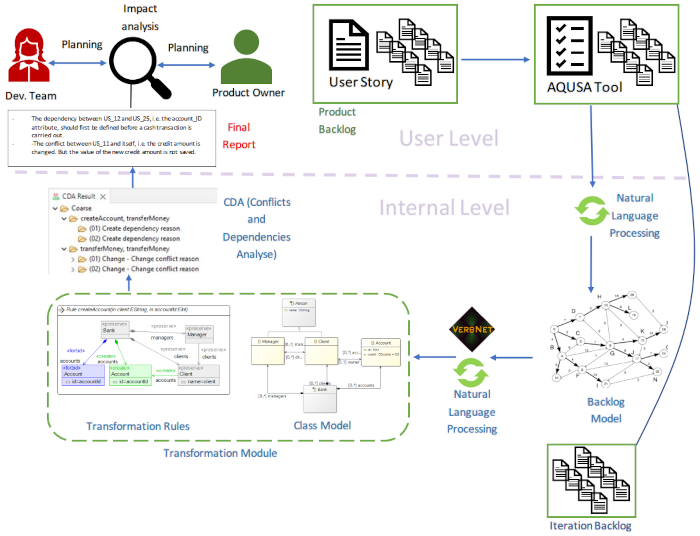
\includegraphics[width=22.8cm, height=16.5cm,left]{1_Big_Picture_v2}
\centering
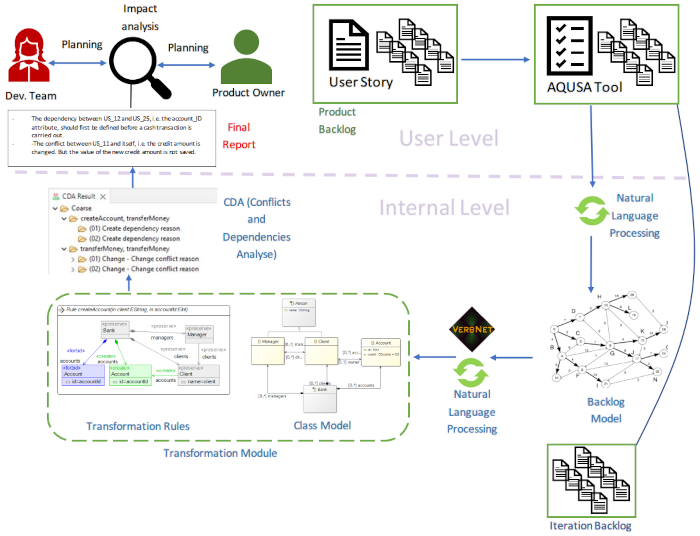
\includegraphics[scale=0.7]{1_Big_Picture_v2}
\caption{Extending backlog model represented by Mosser et al., 2022\cite{mosser2022modelling}}\label{fig:workflow_diagram}
%\restoregeometry
\end{figure}[h]
%\thispagestyle{empty}
%\end{landscape}

\newpage

%\bibliographystyle{abbrv}
%\bibliography{Literatur.bib}

   
\end{document}
